%!TEX root = ../paper.tex

\subsubsection{Data Recipient}
There was a statistically significant difference in VUR for data sent to an application's servers compared to data sent to human recipients. On average, 42\% of participants stated that they would be ``very upset'' if their data was shared with only an application's servers, whereas the VURs for friends (70\%), work contacts (75\%), and the public (72\%) were almost double (Table \ref{recipient-vur}). A chi-square test indicated that these differences were statistically significant (Table \ref{recipient-chi}). However, these effect sizes were small: the largest effect was between work contacts and an app's server ($\phi=0.11$); while the VUR for sharing with work contacts was significantly higher than sharing with friends, the effect size was negligible ($\phi=0.004$). 

We note that this chi-square test violates the assumption of independent observations, since participants responded to multiple scenarios with multiple recipients. But based on the randomization of treatments and large sample size, we do not believe that this significantly impacted our results. Similarly, we are unaware of a more appropriate test, given our data format. Cochran's Q requires binary outcomes (i.e., participants would have had to answer only one question for each data recipient, preventing us from adequately controlling for data type) and a repeated measures ANOVA requires normality (our data was not normally distributed). Nonetheless, we repeated our analysis using only one randomly-selected data point per participant and found that our selected test was robust to this violation. Therefore, we conclude that participants were significantly more concerned about having their data seen by a human versus an application, though differences between specific human groups such as the public, friends, and work contacts were not as significant. 

We do not claim that there are no distinctions between the friends, public, and work contact recipients. People are more comfortable sharing certain data types with certain human data recipients. For instance, participants were significantly uncomfortable sharing if they were lying, nervous, or stressed to work contacts compared to the rest of the data recipients. Participants were much more comfortable sharing phone use and products purchased with an application server than with human recipients. Appendix \ref{sec:recipient-appendix} shows the  complete VUR and rankings of all data types by recipient.

%People have been shown to behave differently, especially in the social arena \cite{dwyer2007trust, gross2005information, fogel2009internet}.

\begin{table}[t]
\begin{center}
\small
\begin{tabular}{| r | l | r | l |c |}
\hline
Rank & Recipient & VUR & sigma & Distribution \\
\hline
1 & Work Contacts & 75.16\% & 0.94 & 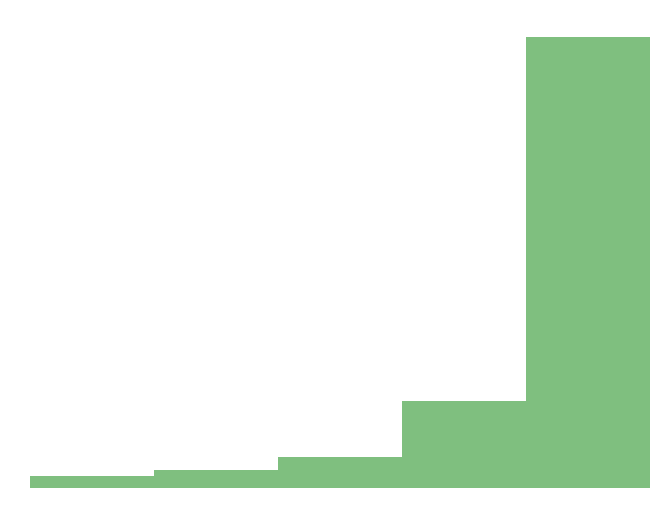
\includegraphics[width = 2cm, height = 0.5cm]{tex-inputs/recipient4/recipient_work} \\
2 & Public & 72.41\% & 0.98 & 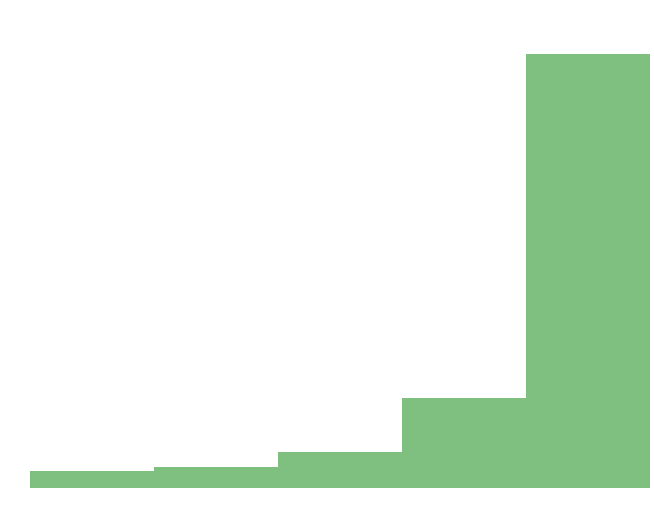
\includegraphics[width = 2cm, height = 0.5cm]{tex-inputs/recipient4/recipient_pub}  \\
3 & Friends & 69.47\% & 1.02 & 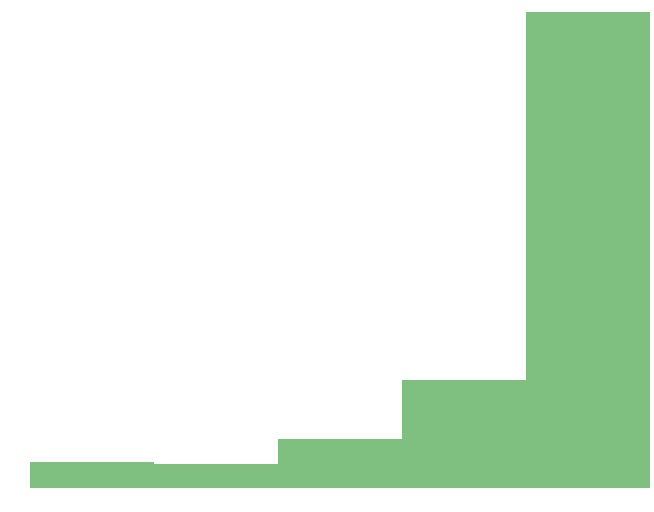
\includegraphics[width = 2cm, height = 0.5cm]{tex-inputs/recipient4/recipient_friends}\\
4 & App's Server & 42.28\% & 1.15 & 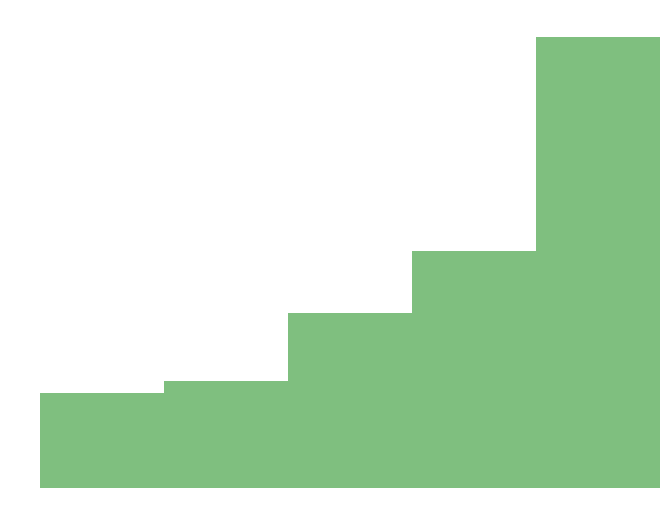
\includegraphics[width = 2cm, height = 0.5cm]{tex-inputs/recipient4/recipient_app}\\
\hline
\end{tabular}
\caption{The overall upset rate for all recipients.}
\label{recipient-vur}
\end{center}
\end{table}

\begin{table}[t]
\small
\begin{center}
\begin{tabular}{|l|r|r|r|r|}
\hline
Recipients	& $\chi^2$ & p-value 	& n & $\phi$ \\
\hline
Work-App	& 565.910 & <0.0001 & 5,083 & 0.111\\
Public-App	& 481.776 & <0.0001 & 5,1988& 0.093\\
Friends-App & 381.653 & <0.0001 & 5,096 & 0.075\\
Friends-Work & 20.39 & <0.0001 & 5,037 & 0.004\\
Friends-Public & 5.41 & <0.0200 & 5,142 & 0.001\\
Work-Public&  5.00 & <0.0253 & 5,129	& 0.001\\
\hline
\end{tabular}
\caption{Results of a chi-square test to examine VUR based on data recipient, across all data points.}
\label{recipient-chi}
\end{center}
\end{table}
